\chapter{Kako goljufati}
\label{ch:kako-gouljufati}

\marginnote{Ta lekcija ima čuden naslov in ni čisto jasno, zakaj smo ga izbrali. Morda nam ti, bralec, lahko poveš, kaj ima ta lekcija z goljufanjem.}Trenutno klasifikacijsko drevo daje odlične rezultate. Zmoti se le v nekaj primerih. Ali lahko podatke tako zelo pokvarimo, da bo drevo neuporabno? Na primer, odstranimo lahko kakršno koli povezavo med genskimi ekspresijami in njihovo funkcijo. Za to bomo uporabili gradnik \widget{Preprocess} in metodo najključnega razporejanja razredov (\textit{randomize class}). Poglejmo si kaos, ki ga ustvari v razsevnem diagramu, kjer smo prej imeli lepe gruče!\marginnote{Zakaj je ozadje razsevnega diagrama popolnoma zeleno?  Kam sta šli drugi dve barvi, modra in rdeča?}

\begin{marginfigure}
    \centering
    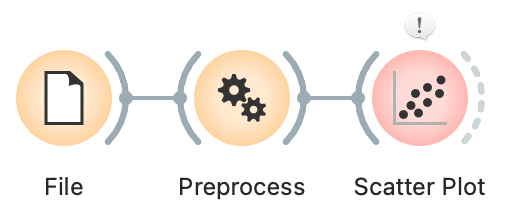
\includegraphics[width=55mm]{workflow1.png}
    \caption{$\;$}
    \label{fig:workflow1}
\end{marginfigure}

\begin{figure}[h]
    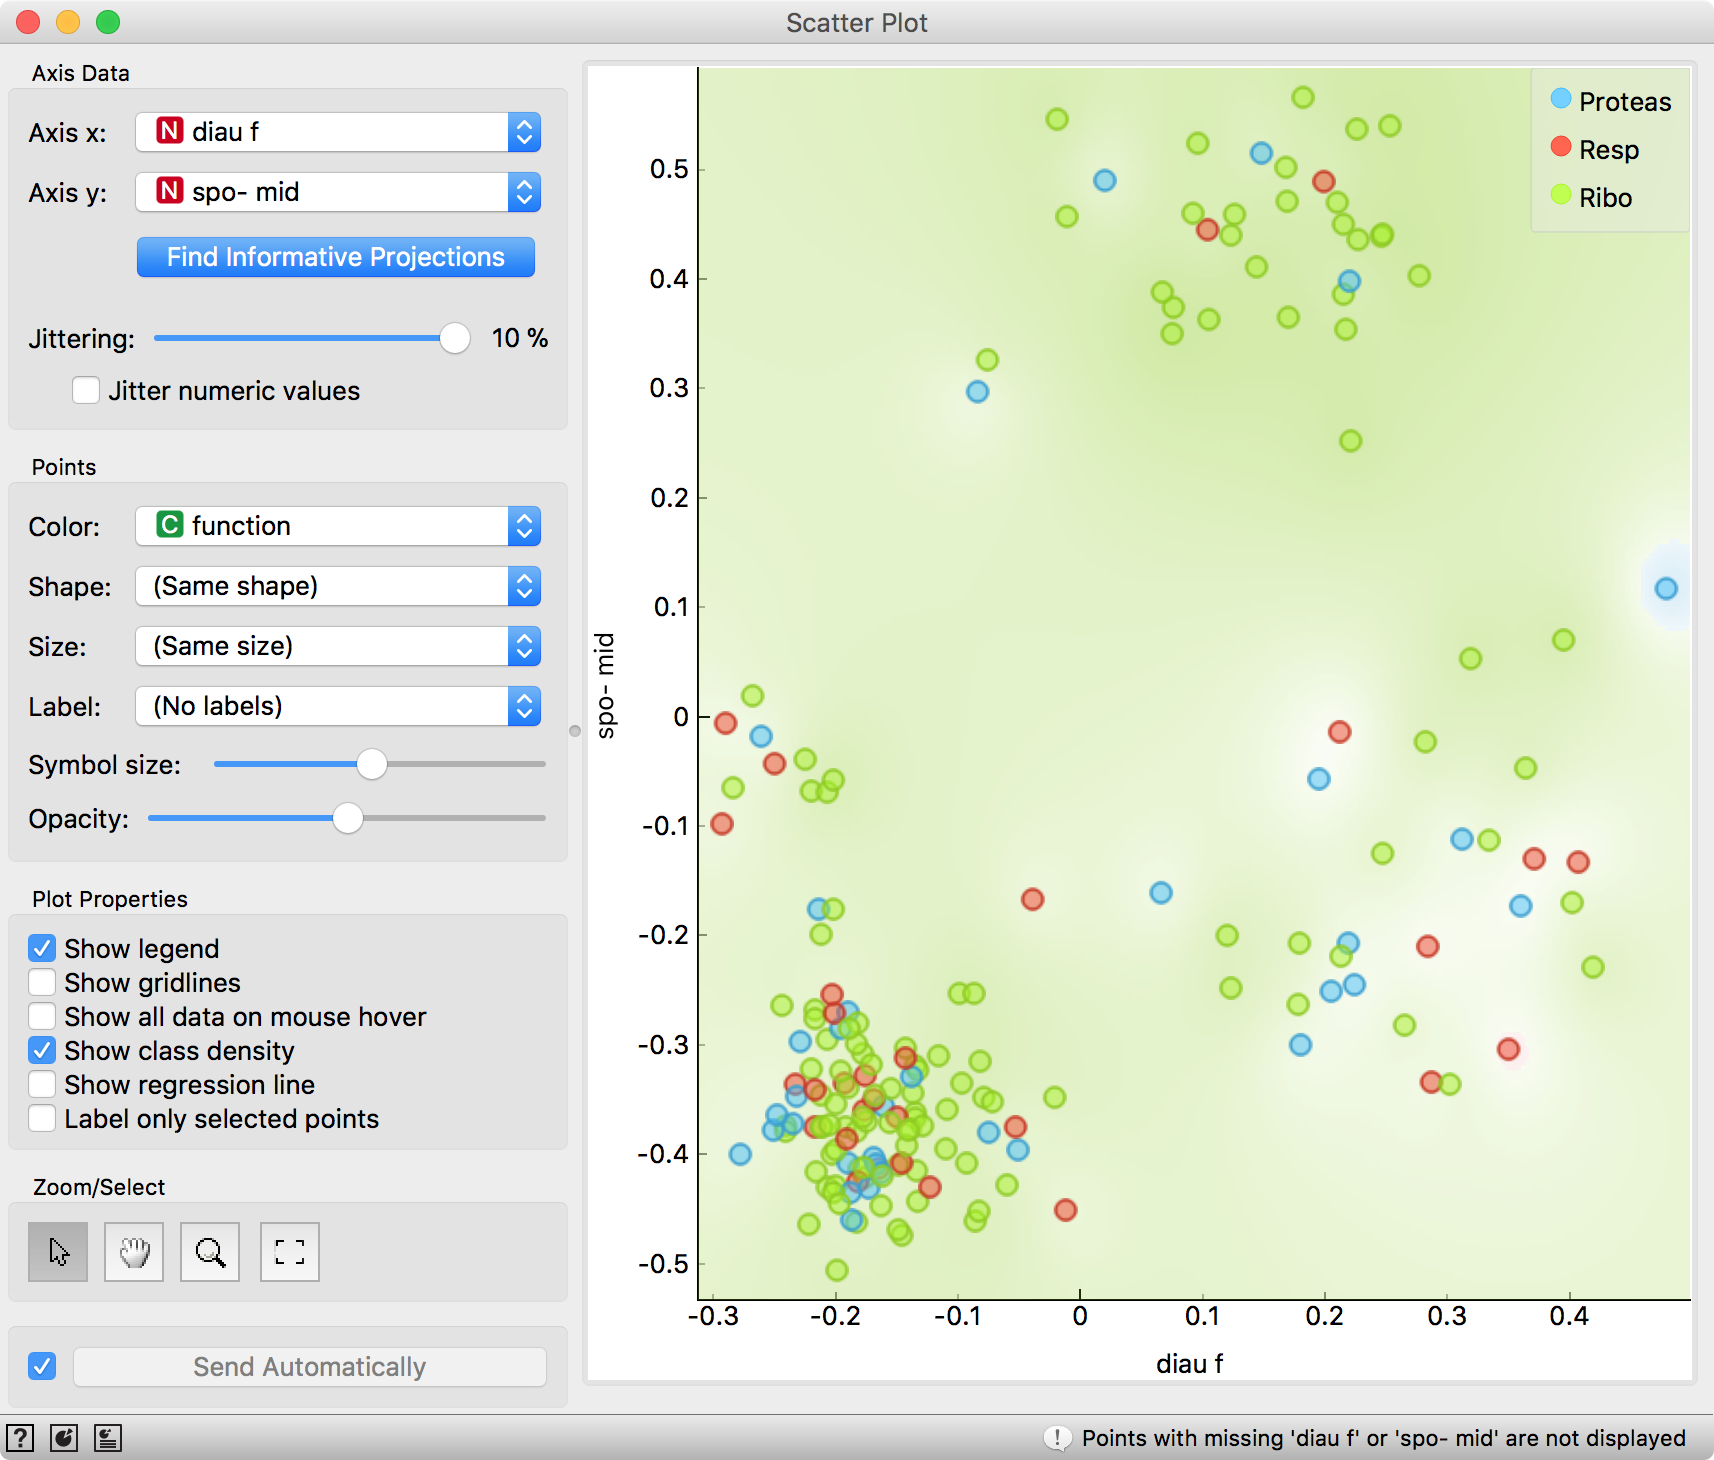
\includegraphics[width=\linewidth]{scatterplot.png}
    \caption{$\;$}
\end{figure}

\begin{wrapfigure}{o}{1.1\textwidth}
    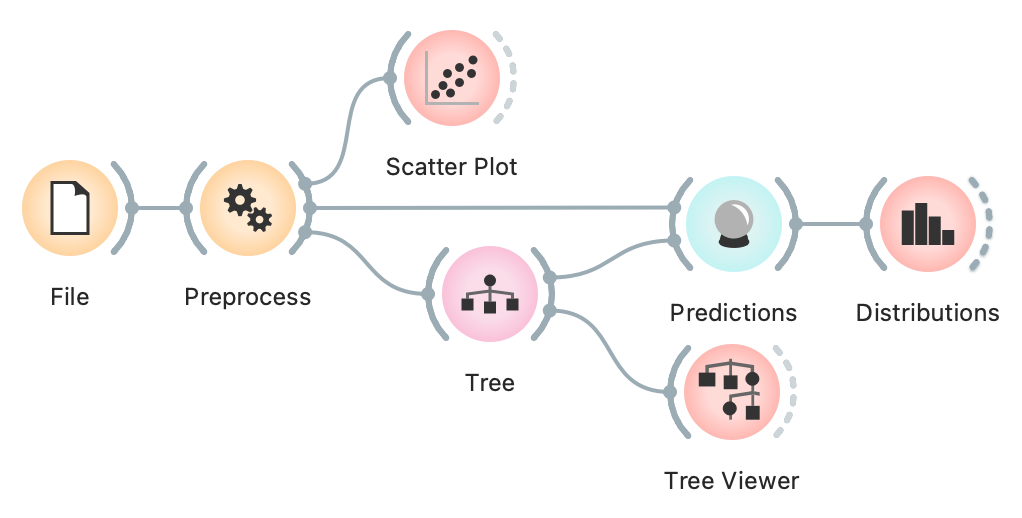
\includegraphics[scale=0.65]{workflow2.png}
    \caption{$\;$}
\end{wrapfigure}

Dobro. Gotovo ni modela, ki bi lahko napovedal tole zmedo. Prepričajmo se. (Ko povezujete Preprocess z gradnikom Tree, bo Orange povezal signala Preprocessor. Tukaj boste morali ročno prevezati povezavo iz \textit{Preprocessed Data} v \textit{Data}. Povezave v dialogu odstranite tako, da kliknete nanje.)

\newpage
\clearpage

In rezultat? Tukaj so naše distribucije:

\begin{figure}[h]
    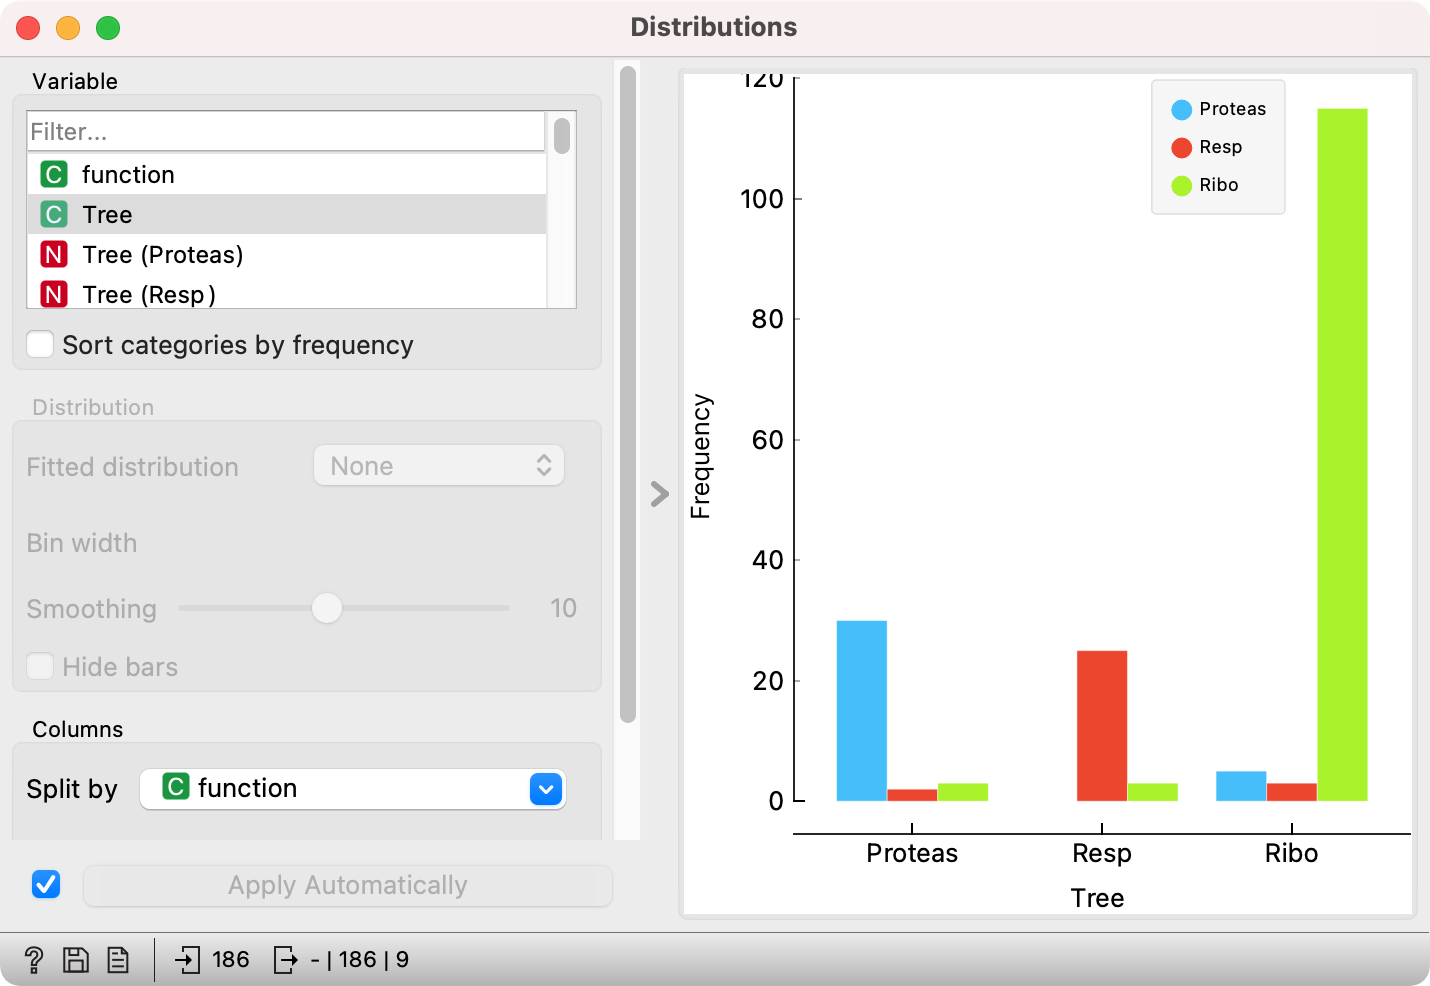
\includegraphics[width=\linewidth]{distributions1.png}
    \caption{$\;$}
\end{figure}

Signali iz gradnika \widget{Data Sampler} nimajo imen, ker smo želeli prihraniti prostor. Data Sampler je razdelil podatke na vzorčne in izven-vzorce (t.i. preostale podatke). Vzorčni so bili poslani v \widget{Tree}, medtem ko so bili preostali poslani direktno v \widget{Predictions}. Nastavite Data Sampler tako, da bosta množici približno enako veliki.

Nadvse nenavadno. Skoraj brez napak. Kako je to mogoče? In to na naključnih podatkih?\marginnote{Signali iz gradnika Data Sampler nimajo imen, ker smo želeli prihraniti prostor. Data Sampler je razdelil podatke na vzorčne in izven-vzorce (t.i. preostale podatke). Vzorčni so bili poslani v Tree, medtem ko so bili preostali poslani direktno v Predictions. Nastavite Data Sampler tako, da bosta množici približno enako veliki.}

Uganko bomo rešili tako, da odpremo Tree Viewer in pogledamo drevo. Koliko vej ima? Ali končne veje vsebujejo veliko primerov?

Očitno si je drevo preprosto zapomnilo vsak primer iz podatkov. Nič čudnega, da so bile napovedi tako dobre. Drevo nima nobenega smisla in je kompleksno, ker si je zapomnilo vse skupaj.

Če je temu tako, če si klasifikator zapomni podatke, ne da bi odkril splošne vzorce, bo na novih podatkih popolnoma zanič. Preverimo. Podatke bomo razdelili na dva dela, na učno in testno množico. Klasifikator bomo naučili na učnih podatkih, točno pa bomo ocenili na testnih.

\begin{figure*}[h]
    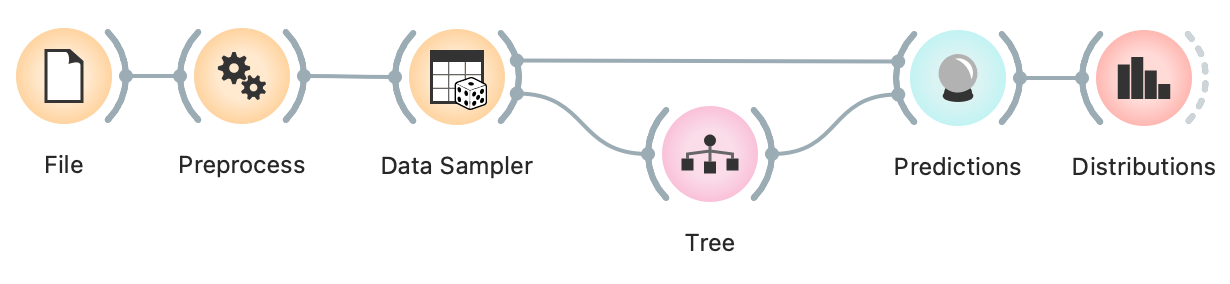
\includegraphics[width=0.9\linewidth]{workflow3.png}
    \caption{$\;$}
\end{figure*}

\newpage
\clearpage

Poglejmo, kako izgleda naš Distributions gradnik po testiranju klasifikatorja na testnih podatkih.\marginnote{Izgleda, da je bila večina genov napovedana kot ribosomnih. Zakaj? Zopet je vse zeleno (tako kot na razsevnem diagramu). Namig: odgovor najdete v gradniku Box Plot.}

\begin{figure}[h]
    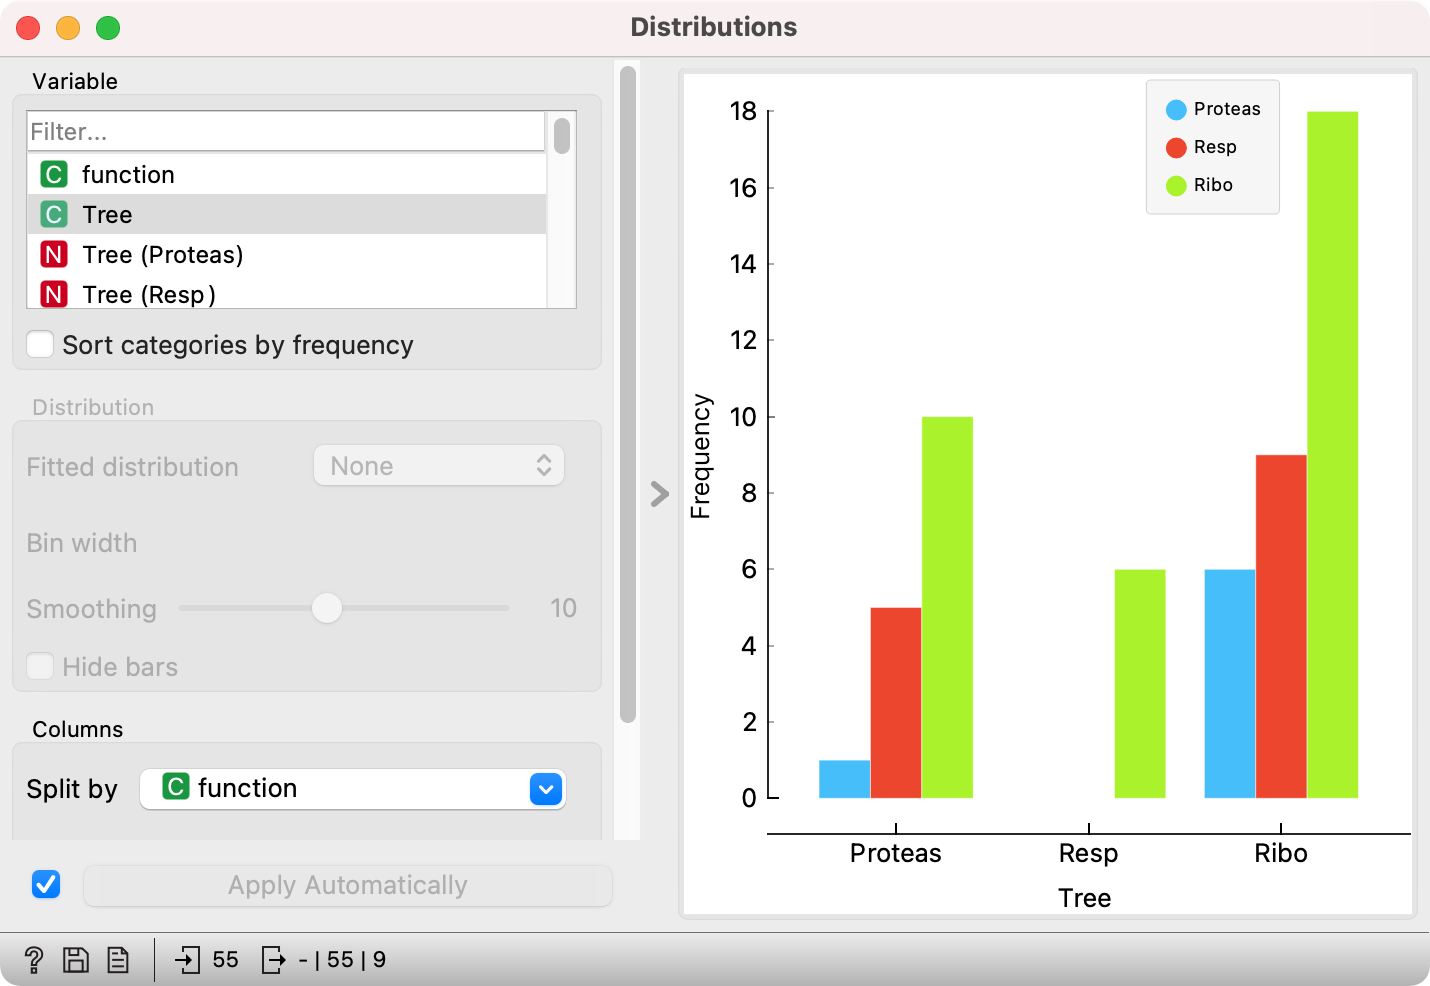
\includegraphics[width=\linewidth]{distributions2.png}
    \caption{$\;$}
\end{figure}

Napovedi funkcije genov so popoln polom. Na naključno zmešanih učnih podatkih naš klasifikator odpove. Končno to, kar smo pričakovli.

Da bi res preizkusili kvaliteto (točnost) klasifikacijske metode, moramo naučiti model na učnih podatkih in ga potem preveriti na testnih. S testom lahko razlikujemo med klasifikatorji, ki si rezultate zapomnijo na pamet, in temi, ki se naučijo splošen model. 

\marginnote{Da bi klasifikator odpovedal, smo morali naključno zmešati samo učne podatke. Poskuite spremeniti delotok tako, da bodo vrednosti razredov premešane zgolj v učnih podatkih, ne pa tudi v testnih.}Učenje ni piflarija. Nasprotno, učenje je odkrivanje vzorcev, ki vladajo podatkovm, in prenašanje teh vzorcev na nove podatke. Da lahko ocenimo točnost klasifikatorja, potrebujemo torej testne podatke. Ta ocena pa ne sme biti odvisna od samo ene delitve podatkov na učne in testne (tudi tukaj je prostor za goljufanje). Nasprotno, postopek testiranja moramo ponoviti večkrat, vsakič z novima učno-testnima množicama in potem poročati o povprečnem rezultatu.